\documentclass{acsman}
\usepackage{float}
\usepackage[dvipdfmx]{graphicx}
\usepackage{url}
\usepackage{amsmath}
\usepackage{subfigure}
\usepackage{titlesec}
\usepackage{tabularx}
\usepackage{booktabs}

\usepackage{multirow}
    \newcolumntype{C}{>{\centering\arraybackslash}X}
    \newcolumntype{L}{>{\raggedright\arraybackslash}X}
    \newcolumntype{R}{>{\raggedleft\arraybackslash}X}



\pagestyle{myheadings}

\setcounter{page}{
%%%   ページ数の設定 (Page number)   %%%
1
%%%%%%%%%%%%%%%%%%%%%%%%%%%%%%%%%%%%%%%%
}

\begin{document}
\noindent
\twocolumn[
\Large
\begin{flushright}
\end{flushright}



\begin{center}
%%%   題目 (Title)   %%%
{\bf
修 士 論 文 要 旨

Summary of the Master's Thesis
}
\end{center}
\normalsize
\vspace{\baselineskip}
\normalsize

%\renewcommand{\arraystretch}{1.5}
\begin{tabularx}{\textwidth}{|c|X|c|X|}
\hline
学 生 番 号 & \multirow{2}{*}{M225163} & プログラム  &\multirow{2}{*}{情報科学プログラム} \\
Student ID Number& &Program& \\
\hline
氏 名  & \multirow{2}{*}{張 邦林} & 主 指 導 教 員  &\multirow{2}{*}{中野 浩嗣} \\
Name& &Supervisor& \\
\hline
論 文 題 目 & \multicolumn{3}{c|}{\multirow{2}{*}{Watercolor Image Generation Based on Diffusion Model}}  \\
Thesis Title& \multicolumn{3}{c|}{} \\
\hline
\end{tabularx}



\normalsize
\vspace{2\baselineskip}
]
%%%  概要 (Abstract)   %%%
\begin{abstract}
With the development of deep learning, the application of deep learning in image generation is becoming more and more widespread. Especially the generation of images in various special styles, such as oil painting style, sketch style and watercolor style. However, existing research on watercolor style image generation is often achieved by style conversion, which limits the creative ability of the model. At the same time, the models do not simulate the watercolor effect well.

In this study, in order to solve the above problems. Firstly, a high-quality watercolor image dataset is produced and used for model training. In order to achieve the purpose of generating high quality watercolor images. Starting from Vision Transformer and diffusion model, this study abandons the U-Net structure commonly used in diffusion model and redesigns the network structure of diffusion model based on Vision Transformer. Compared with the existing model, the quality of watercolor image generation is improved.
\end{abstract}

%%%  本文 (Text)   %%%

\section{Introduction}
The rapid development of deep learning techniques has not only led to remarkable achievements in the traditional fields of computer vision and natural language processing, but has also demonstrated its potential in the creation of art. One notable application is the use of deep learning to generate watercolor images, watercolors are known for their distinctive brushstrokes, soft color transitions, and unique style, and deep learning techniques are able to simulate and reproduce this traditional art form in an unprecedented way. However, due to the characteristics of watercolor images, popular deep learning generation models often fail to achieve satisfactory results. This has driven the development of specialized generative network architectures for watercolor image generation. We created a high-quality watercolor image dataset and designed a new network specifically for the task of watercolor image generation.

Additionally, the network structures used in this study are categorized based on their characteristics. The current mainstream generative models include Generative Adversarial Networks (GAN) \cite{goodfellow2020generative} and diffusion models. Among these, GAN have gained attention due to their widespread application but face several issues such as mode collapse, making it challenging to generate high-quality images. Given these challenges, this study decided to abandon the use of GAN in favor of the more stable diffusion models. Diffusion models generate high-quality and diverse images by progressively adding noise to the images and learning the denoising process. Compared to GAN, diffusion models perform better in terms of stability and generative effects, and they are better at reconstructing and simulating the characteristics of images.

Diffusion models can maintain high levels of detail and structure when generating images, preserving the original image's texture and color transitions. Through this method, we aim to simulate the characteristics of watercolor paintings, including color blending, edge blurring, and texture effects, to ensure that the generated watercolor images exhibit excellent visual and artistic qualities.

\section{Related Work}\label{sec:related work}
\subsection{Vision Transformer}
Vision Transformer model (ViT) \cite{dosovitskiy2020image} architecture typically consists of components such as a linear embedding layer, a self-attention layer, a fully-connected layer, a feed-forward network layer, and residual connectivity with Layer Normalization.

Unlike traditional convolution-based approaches, Vision Transformer proposes a new paradigm for visual processing. The image is segmented into a series of fixed-size blocks, and the relationships between the blocks are established through a multi-head attention mechanism. The core of this idea is to view the image as a sequence rather than a grid, allowing the model to better capture global information while reducing the number of parameters and computational complexity.

The Multi-Head Attention mechanism allows the model to focus on information at different locations in parallel, effectively dealing with long-range dependencies. ViT performs well when dealing with large-scale image data, with a relatively small number of parameters compared to traditional convolutional networks, providing better scalability. Since it does not rely on a fixed local receptive field, ViT is more flexible in handling images of different sizes and application areas.

\subsection{Diffusion Model}
The key idea of Diffusion Probabilistic Models \cite{ho2020denoising} is to gradually evolve a simple noise distribution into a target data distribution through a diffusion process.Specifically, the basic assumption of Diffusion Probabilistic Models is that an initial simple probability distribution, usually Gaussian (Gaussian noise image). It gradually evolves into a target data distribution (Generated image) through a series of probabilistic diffusion steps. This process can be accomplished by iteratively applying the diffusion operation. 
\begin{figure}[h]
    \centering
    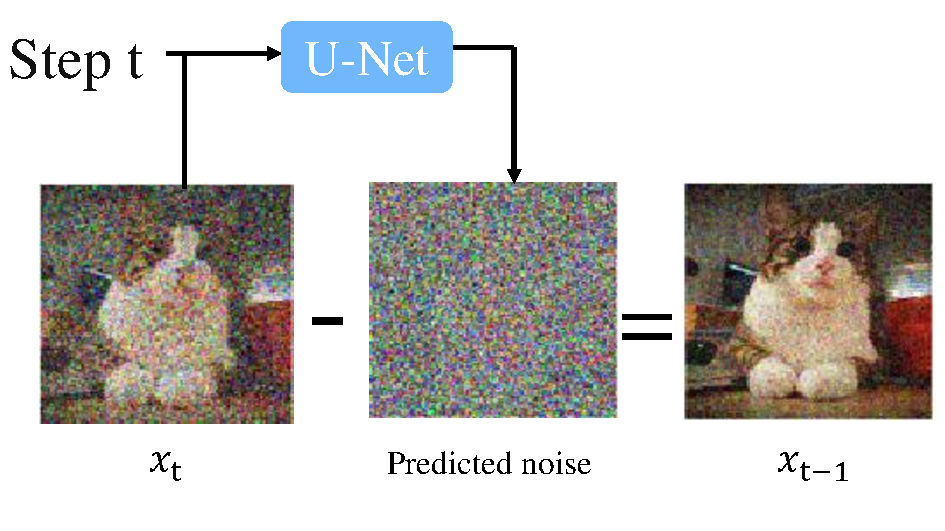
\includegraphics[width=8cm]{image/DDPM.pdf}
    \caption{DDPM single execution process}
    \label{fig:DDPM}
\end{figure}

As shown in Figure \ref{fig:DDPM}, at each step, by removing some of the noise, the current distribution evolves into the distribution for the next step. By performing multiple steps, the model learns how to generate samples (Generated image) that match the target data distribution from a simple distribution (Gaussian noise image), as shown in Figure \ref{fig:DDPM1}.
\begin{figure}[h]
    \centering
    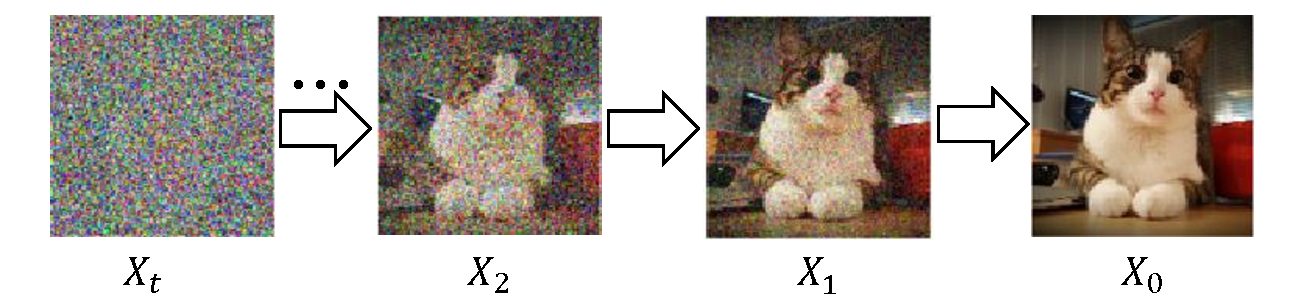
\includegraphics[width=8cm]{image/DDPM1.pdf}
    \caption{Image generation process for DDPM}
    \label{fig:DDPM1}
\end{figure}

Advantages of diffusion models is that they do not require adversarial training like Generative Adversarial Networks (GAN) \cite{goodfellow2020generative}, nor do they involve the complex inference processes of Variational Autoencoders (VAE) \cite{kingma2013auto}. This simplified training method makes diffusion probabilistic models easier to train in certain cases. GAN often face issues such as mode collapse and training instability, while VAE may involve high-dimensional integration calculations in their inference processes, adding to the complexity and difficulty of training the models. In contrast, diffusion models can be trained more smoothly and efficiently by gradually introducing noise and learning the denoising process.

Since their initial proposal in 2015, diffusion probabilistic models have made significant advancements in backbone network structures. from the MLP used by Jascha in 2015 \cite{sohl2015deep}, to Song Yang's work in 2019 when he first constructed a diffusion model using the U-Net \cite{song2019generative}, and a series of improvements to the U-Net by subsequent works. Such as the DDPM \cite{ho2020denoising}, and the Imagen \cite{saharia2022photorealistic}. Imagen and many other works have made a series of improvements to U-Net. At present, most studies on diffusion probability modeling still use U-Net as the backbone network.

\begin{figure*}[thb]
    \centering
    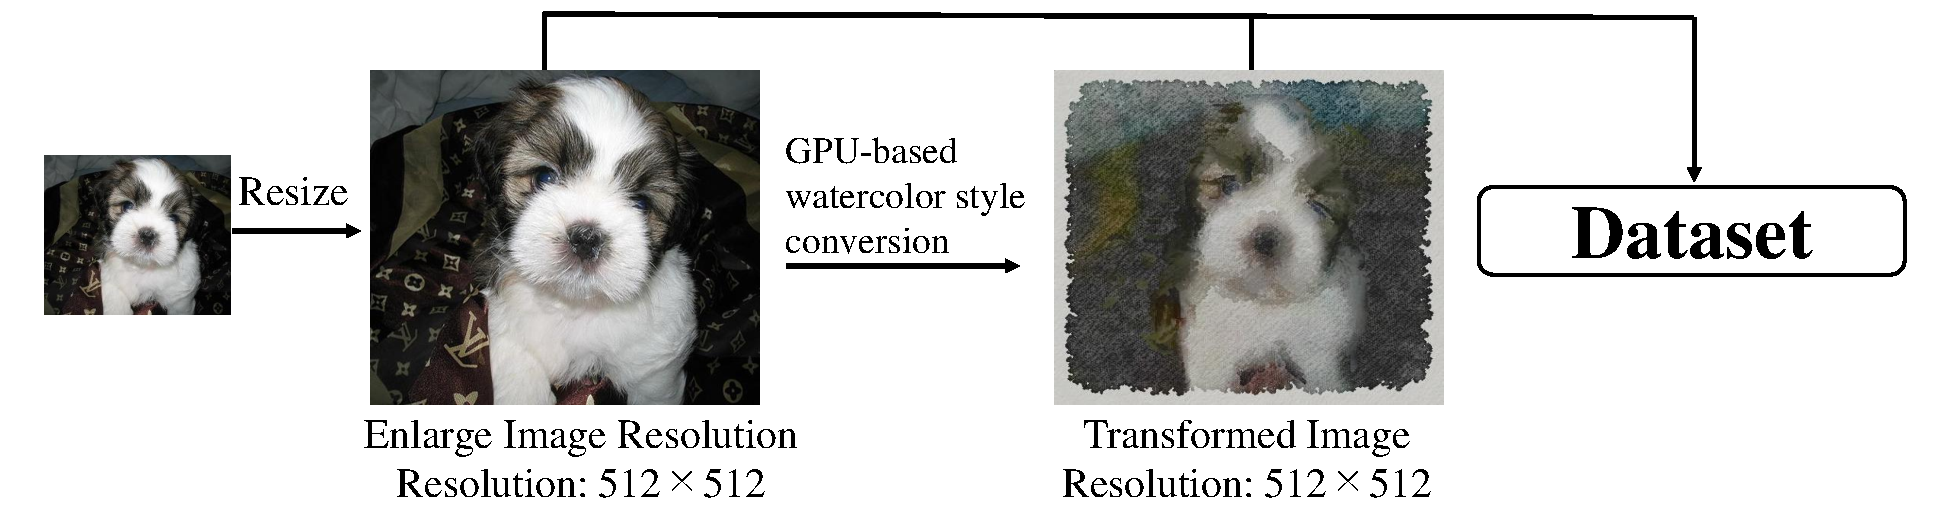
\includegraphics[width=14cm]{image/gpu.pdf}
    \caption{The process of watercoloring ImageNet image}
    \label{fig:gpu}
\end{figure*}

\section{Datasets}\label{sec:dataset}
\subsection{Watercolor Dataset}
The watercolor dataset used in this study was personally collected based on the ImageNet dataset. ImageNet is a large-scale image dataset initially created by Fei-Fei Li and others at Stanford University. It contains over a million high-resolution images spanning a thousand different categories, with each category typically including hundreds to thousands of images \cite{deng2009imagenet}. 

In this study, images from selected categories of the ImageNet dataset were converted to watercolor images using GPU methods. Ultimately, the resulting dataset comprised 35 categories, each with approximately 2,000 images. Each image had a resolution of 512$\times$512, and the total dataset included 68,550 images.


\subsection{Methods of Dataset Collection}

Due to the current lack of open-source watercolor datasets, this study used GPU methods to collect watercolor images as the dataset. The GPU method itself does not depend on a specific dataset, meaning it can convert input images into watercolor images. This method can simulate relatively realistic watercolor effects but still requires input images.

In this study, the dataset images were collected using this method, and the specific process is Figure \ref{fig:gpu}. First, the resolution of images from the ImageNet dataset was increased from 256$\times$256 to 512$\times$512. This is because the performance of the aforementioned GPU method deteriorates significantly at lower resolutions. Then, the images with the increased resolution were converted into watercolor images using the GPU method. This resulted in watercolor images along with their corresponding original ImageNet images.


To ensure the model retains more semantic information during the generation process, we adopted a unique approach when constructing the dataset. This approach involves using both watercolor styled images and the original ImageNet images. Specifically, this means that for each category, the dataset includes not only the original images but also their corresponding watercolor styled images. These images appear in pairs. This dual image processing method helps the model better understand and retain key semantic features during training, thereby improving the quality and accuracy of the generated results.

\section{Proposed Method}\label{sec:method}
To achieve the goal of generating high-quality images and reducing the computational load of the model, this study's model comprises two networks. As shown in Figure \ref{fig:overall}, the Transformer model and the AutoencoderKL model. During the image generation process, the Transformer model first generates specific feature maps from random noise, guided by labels. Then, the AutoencoderKL model decodes these feature maps generated by the Transformer model into images.

\begin{figure}[H]
    \centering
    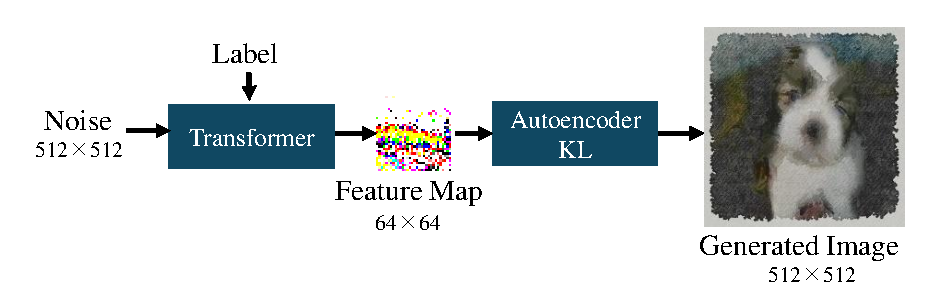
\includegraphics[width=8.2cm]{image/overall.pdf}
    \caption{Overall structure}
    \label{fig:overall}
\end{figure}

\subsection{Transformer Model}
To generate high-quality watercolor images, this study abandoned the commonly used U-Net network in traditional diffusion models and instead reconstructed a network based on the Vision Transformer model as the backbone of the diffusion model, as shown in Figure \ref{fig:traM}. The Attention structure of the Transformer model possesses stronger global perception capabilities, a feature particularly important in the process of generating watercolor images. By leveraging this structure, the watercolor image generation process can more effectively simulate the diffusion and blending effects of watercolor pigments, thereby enhancing the overall texture and detail expressiveness of the images. Compared to traditional methods, the Vision Transformer-based network not only excels in simulating watercolor effects but also significantly improves the quality and realism of the generated images.
\begin{figure*}[tbp]
    \centering
    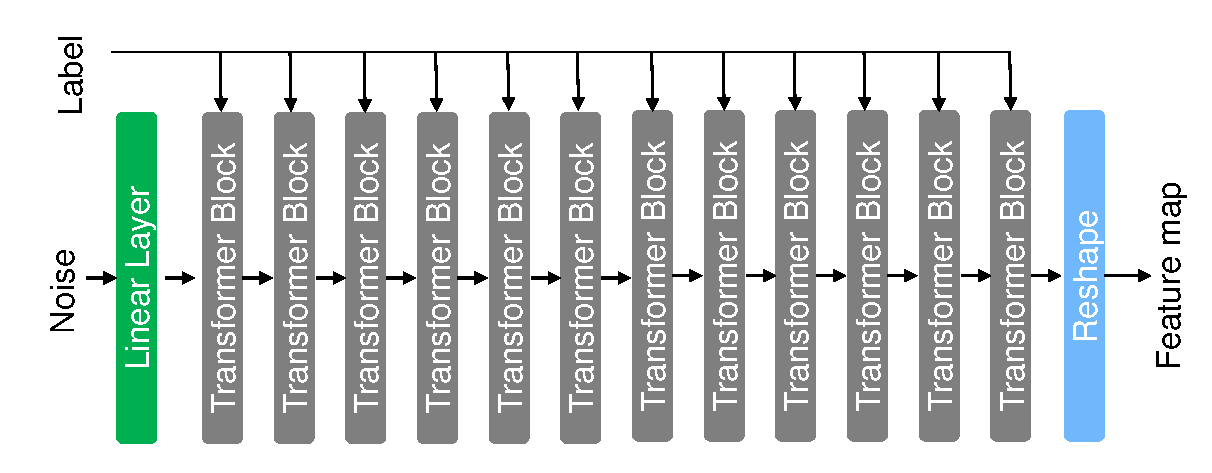
\includegraphics[width=16cm]{image/traM.pdf}
    \caption{Transformer model structure}
    \label{fig:traM}
\end{figure*}
\subsection{Transformer Block}
The design of the Transformer Block generally follows the linear structure of the traditional Vision Transformer, as shown in Figure \ref{fig:Transformer_Block}. The difference in this study's Transformer Block design is the replacement of the original MLP layer with a Feed-Forward layer, using the MLP to input label information. To improve the model's performance, the number of Multi-Head Attention layers (MH-Attention) was increased, and the Multi-Head Attention layers and Feed-Forward layers were used in pairs. This is because the Multi-Head Attention layer has relatively weak local perception and non-linear capabilities, which are compensated for by the Feed-Forward layer. The Multi-Head Attention layer, through the parallel processing of multiple attention heads, can better capture the global information of the input data. Meanwhile, the Feed-Forward layer, through non-linear transformations, enhances the model's ability to handle complex patterns and features.

\begin{figure}[H]
    \centering
    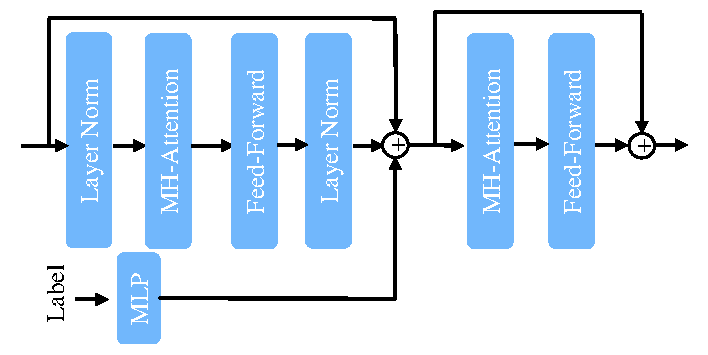
\includegraphics[width=8cm]{image/Transformer_Block_sum.pdf}
    \caption{Transformer block structure}
    \label{fig:Transformer_Block}
\end{figure}

\subsection{Feed Forward Layer and MLP}
The structure of the Feed Forward Layer designed in this study is shown in Figure \ref{fig:FFL}. The main function of the Feed Forward Layer is to compensate for the shortcomings of the Attention layer in terms of non-linear capability and local perception.
\begin{figure}[H]
    \centering
    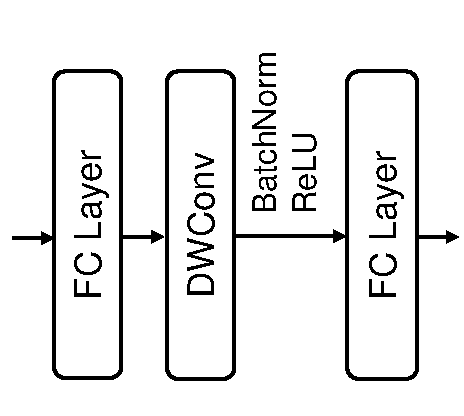
\includegraphics[width=5.5cm]{image/FFL_sum.pdf}
    \caption{Feed Forward Layer structure}
    \label{fig:FFL}
\end{figure}
The structure of the Feed Forward Layer designed in this study is shown in Figure \ref{fig:FFL}. The main function of the Feed Forward Layer is to compensate for the shortcomings of the Attention layer in terms of non-linear capability and local perception.

MLP (Multilayer Perceptron) is a simple neural network structure, usually consisting of several fully connected layers and activation functions. In the original Vision Transformer, an MLP was often connected after the Attention layer to introduce nonlinear capabilities to the model. In this study, an MLP is used to input label data into the model. The structure of the MLP is shown in Figure \ref{fig:MLP}. This MLP structure adopts a combination of fully connected layers and Layer Normalization + SiLU. 

\begin{figure}[H]
    \centering
    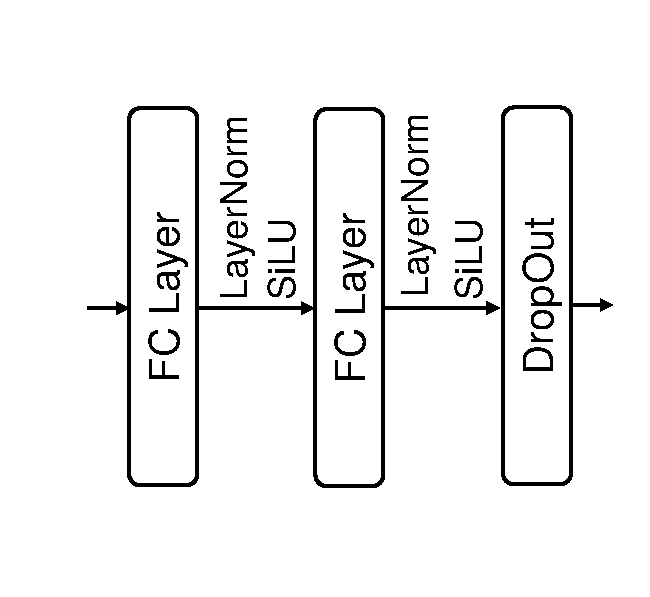
\includegraphics[width=5.5cm]{image/MLP_sum.pdf}
    \caption{MLP structure}
    \label{fig:MLP}
\end{figure}


\section{Results}\label{sec:result}
\subsection{Train Details and Valuation Metric}
To train this model, NVIDIA RTX A6000$\times$2 was used. and the batch size was set to 16, the learning rate was 1e-4, and the optimizer was selected as AdamW. A total of 1500 epochs were trained, and checkpoints were saved at every 300 epochs. 
Regarding evaluation metrics, this study uses FID (Fréchet Inception Distance) \cite{FID} as an objective evaluation metric. Additionally, questionnaire are used as a subjective evaluation metric. 
\subsection{Comparison with GPU method}
In the previous section, a GPU method was used to generate the dataset \cite{huang2021gpu},
comparison of the generated images was carried out. The image style conversion by GPU method (green box is original image). and generated images with using the model in this study. Approximate images were generated for ease of comparison (beach image). As shown in Figure \ref{fig:wGPU}.

\begin{figure}[htbp]
    \centering
    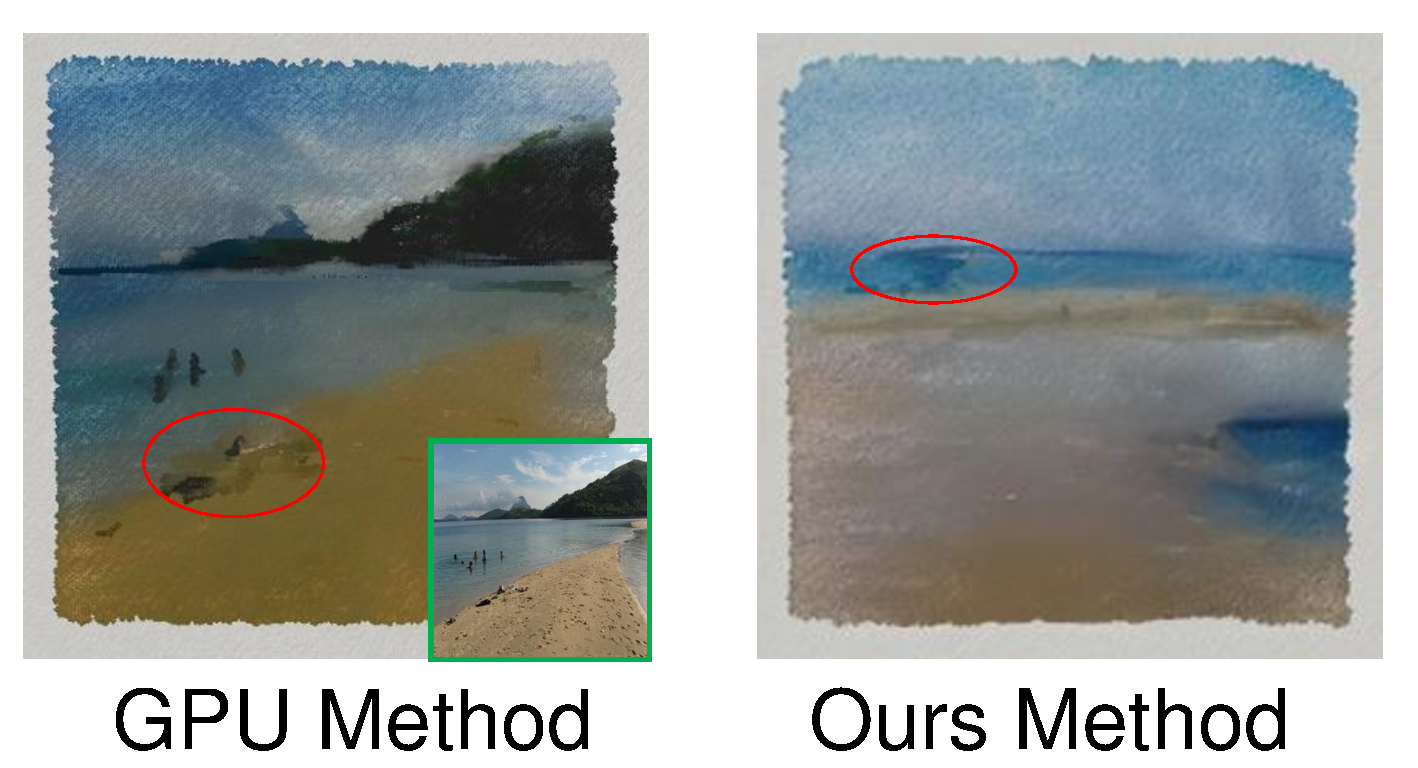
\includegraphics[width=8cm]{image/wGPU.pdf}
    \caption{Comparison of the generated image with GPU generation method (Beach)}
    \label{fig:wGPU}
\end{figure}

Compared to the GPU method generated images, the model excels particularly in color blending, especially in the red-circled areas, showcasing the natural merging effect characteristic of watercolor paintings. Additionally, the blurred edges in the image make the overall picture softer and more realistic.


\subsection{Comparison with DDPM and LDM}
Comparing the above three models generates images (Agaric) as shown in Figure \ref{fig:eva}. The model in this study achieved the best watercolor simulation subjectively. Looking closely at the generation results, this study's model has a better reconstruction of the target within the image, and the unique features of watercolor images such as color diffusion and color fusion appear at the line edges of the image.
\begin{figure}[h]
    \centering
    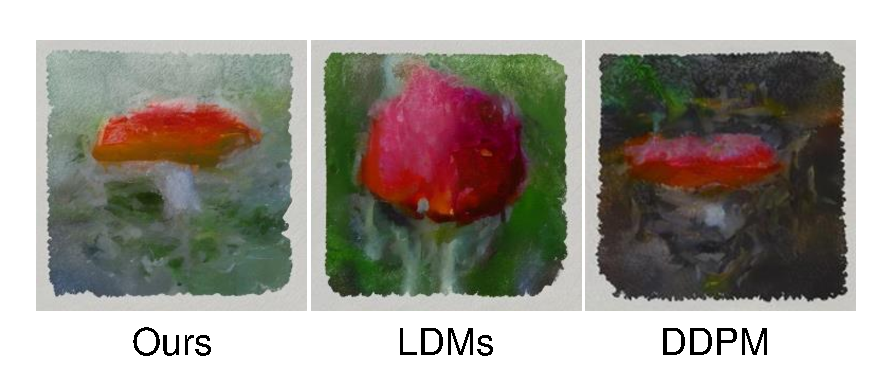
\includegraphics[width=8cm]{image/eva.pdf}
    \caption{Comparison of the generated image (Agaric)}
    \label{fig:eva}
\end{figure}
In terms of objective evaluation, the generated results of the model were objectively evaluated using FID \cite{FID}. As shown in Table \ref{tab:fid}, the model in this study obtained the lowest FID compared to the original Denoising Diffusion Probabilistic Models (DDPM) \cite{ho2020denoising} and Latent Diffusion Models (LDM) \cite{rombach2022high}.

\begin{table}[htbp]
  \centering
  \caption{Objective evaluation}
  \label{tab:fid}
  \begin{tabular}{c c}
    \hline
    Model & FID  \\
    \hline
    DDPM & 73.933  \\
    LDM & 67.261\\
    Ours & 64.332  \\
    \hline
  \end{tabular}
\end{table}

In terms of subjective evaluation, this study collected a total of 11 valid questionnaires. The results in Table \ref{tab:point} indicate that the DDPM model's score is significantly lower compared to the other models, with a score of 143. In contrast, the LDM model received a score of 220, while our model slightly outperformed the LDM model in user ratings, achieving a score of 297. These results are consistent with the objective FID evaluation and further validate the superiority of our model in generating high-quality watercolor images from the users' perspective. These subjective evaluation results further demonstrate the advantages of our model in generating watercolor images.

\begin{table}[htbp]
  \centering
  \caption{Subjective evaluation}
  \label{tab:point}
  \begin{tabular}{c c}
    \hline
    Model & Sum Points  \\
    \hline
    DDPM & 143  \\
    LDM & 220  \\
    Ours & 297  \\
    \hline
  \end{tabular}
\end{table}

\section{Conclusion}
In this study, we created a high-quality watercolor dataset and designed a neural network based on the Transformer architecture specifically for watercolor image generation. The detailed design of the model's framework allows for the generation of images according to labels. The generated images retain the characteristics of watercolor paintings, such as color blending and diffusion effects. Both objective metrics and subjective evaluations indicate that the performance of our model in generating watercolor images slightly surpasses that of popular diffusion models based on the U-Net structure.


%%%  参考文献 (Thebibliography)   %%%
\bibliographystyle{IEEEtran}
\bibliography{sample}

\end{document}
